\documentclass[12pt,a4paper]{article}
\usepackage{kotex}
\usepackage{hyperref}
\usepackage{amssymb}
\usepackage{amsmath,amsthm,amsfonts,amscd}
\usepackage[utf8]{inputenc}
\usepackage{geometry}
\usepackage{titling}
\usepackage{titlesec}
\usepackage{xcolor}
\usepackage{graphicx}
\usepackage{fancyhdr}
\usepackage{lipsum} % for generating sample text
\usepackage{wallpaper}
\usepackage{tabularx}
\usepackage{booktabs}

\usepackage{tikz}
\usepackage{pgf-pie}

% Define custom colors
\definecolor{darkblue}{RGB}{25,25,112}  % Midnight Blue
\definecolor{lightblue}{RGB}{173,216,230}  % Light Blue

\usepackage{geometry}
\geometry{a4paper,left=.7in,right=.7in,top=1in,bottom=1in,heightrounded}
% Header and Footer
\pagestyle{fancy}
\fancyhead{}
\fancyhead[L]{\textcolor{darkblue}{\bf P.A.N.D.A's PUBAO: Discrete Logarithm Calculator Development}}
\fancyfoot{}
\fancyfoot[C]{\thepage}
\renewcommand{\headrulewidth}{0.5pt}
\renewcommand{\footrulewidth}{0.5pt}
\renewcommand{\headrule}{\hbox to\headwidth{\color{lightblue}\leaders\hrule height \headrulewidth\hfill}}
\renewcommand{\footrule}{\hbox to\headwidth{\color{lightblue}\leaders\hrule height \footrulewidth\hfill}}

% Title Styling
\pretitle{\begin{center}\Huge\color{darkblue}\bfseries\scshape}
	\posttitle{\end{center}\vskip 0.5em}
\preauthor{\begin{center}\large\color{lightblue!50!black}\scshape\lineskip 0.5em}
	\postauthor{\end{center}}
\predate{\begin{center}\color{darkblue}\large\scshape}
	\postdate{\end{center}}

% Section Styling
\titleformat{\section}
{\color{darkblue}\normalfont\Large\bfseries\scshape}
{\color{darkblue}\thesection}{1em}{}
\titleformat{\subsection}
{\color{lightblue!50!black}\normalfont\large\bfseries\scshape}
{\color{lightblue!50!black}\thesubsection}{1em}{}

%Tcolorbox
\usepackage[most]{tcolorbox}
\tcbset{colback=white, arc=5pt}

% Font Selection
\renewcommand*\familydefault{\sfdefault} 

% Background Image
%\ULCornerWallPaper{1}{panda3.png} % Replace 'background.jpg' with your image file 

% Title, Author, Date
\title{P.A.N.D.A's PUBAO: \\Discrete Logarithm Calculator Development}
\author{\textcolor{lightblue!50!black}{\bf 지용현, 김예찬, 문예찬, 유근오}}
\date{\today}

\begin{document}
	
	\maketitle
	\thispagestyle{empty}  % Removes header/footer on first page
	\begin{figure}[h!]
		\centering
		
\includegraphics[scale=.5]{panda4.png}
	\end{figure}
	\newpage  % Ensures that content starts on the second page
	
	\section*{Abstract}
	Abstract: Development of a Large Integer Arithmetic Library and Discrete Logarithm Calculator Using Shanks' Algorithm
	
	Problem: In the realm of cryptography and number theory, computing the discrete logarithm is a fundamental challenge. For large integers, traditional computational methods are either inefficient or infeasible. The vast applications of discrete logarithm in cryptographic systems demand an effective solution for calculating it efficiently, especially for big numbers.
	
	Solution: This project introduces a comprehensive large integer arithmetic library, designed to efficiently handle and compute vast numbers. Leveraging this library, we have developed a specialized calculator to solve discrete logarithm problems, using the renowned Shanks' (or baby-step giant-step) algorithm. Shanks' method divides the problem into more tractable smaller parts, providing a considerable speedup over naive techniques, especially when our large integer arithmetic library optimizes computations.
	
	Impact: The developed large integer arithmetic library offers versatility, not just limited to our calculator but expandable to other computational problems requiring big number arithmetic. The discrete logarithm calculator, by capitalizing on Shanks' algorithm, provides an invaluable tool for researchers, cryptanalysts, and educators. By simplifying and expediting the calculation of discrete logarithms, this project aids in enhancing cryptographic practices, facilitates research in number theory, and serves as an educational platform for advanced mathematical concepts.
	\tableofcontents
	\newpage
	\section{Team Overview}
	\begin{itemize}
		\item \textbf{Team Name:} \textcolor{magenta}{\bf P.A.N.D.A. 
		\text{\small(Programmers Aspiring to Navigate Digital Arithmetic)} }
		\item \textbf{Project Name:} \textcolor{magenta}{\bf PUBAO \text{\small(P.A.N.D.A.'s Unbounded Big Arithmetic Operations)}}
		\item \textbf{Member:}
		\begin{itemize}
			\item[$\blacktriangleright$] \textcolor{darkblue}{\bf 지용현 (Leader)}
			\begin{itemize}
				\item[-] \textbf{Strategic Planning:} 프로젝트의 전반적인 방향을 설정하고 목표과 목적이 프로젝트 비전을 이끌어 나간다.
				\item[-] \textbf{Algorithm Implementation:} 계산 알고리즘의 실제 구현과 더불어 라이브러리와의 원활한 통합을 진행한다.
			\end{itemize}
			\vspace{5pt}
		\item[$\blacktriangleright$] \textcolor{darkblue}{\bf 김예찬 (Validator) }
		\begin{itemize}
			\item[-] \textbf{Quality Assurance:} 개발된 모듈이 버그가 없는지 확인한다.
			\item[-] \textbf{Feedback Loop:} 사용자 피드백을 수집하고 지속적인 개선을 촉진한다.
		\end{itemize}
		\vspace{5pt}
			\item[$\blacktriangleright$] \textcolor{darkblue}{\bf 문예찬 (Builder)}
		\begin{itemize}
			\item[-] \textbf{Core Development:} 필수 모듈 개발을 주도하고, 성능이 프로젝트 요구 사항에 부합하는지 확인한다.
			\item[-] \textbf{Integration:} 큰 정수 연산 라이브러리를 계산기와 통합하여 원활하고 오류 없는 작동을 보장한다.
		\end{itemize}
		\vspace{5pt}
			\item[$\blacktriangleright$] \textcolor{darkblue}{\bf 유근오 (Intern)}
		\begin{itemize}
			\item[-] \textbf{User Interface Design:} 계산기의 사용자 인터페이스를 디자인하고 개발하여 사용자 친화적이고 직관적인 디자인을 설계한다.
			\item[-] \textbf{Testing:} 개발된 라이브러리의 정확성과 효율성을 보장하기 위해 다양한 시나리오를 테스트 단계에서 테스트한다. 
		\end{itemize}
		\end{itemize}
	\end{itemize}
	
	\section{Develop Environment}
	\begin{itemize}
		\item Language: C17
		\item Compiler: gcc (Ubuntu 11.4.0-1ubuntu1~22.04) 11.4.0
		\item Development Tools
		\begin{itemize}
			\item SageMath version 9.5
			\item valgrind-3.18.1
			\item OpenSSL 3.0.2 15 Mar 2022
			\item GPT-4
			\item Notion:\\ \url{https://hacker-code-j.notion.site/2023-Fall-AAP-Team-3-P-A-N-D-A-FUBAO-8a09720a080c4ad5859913331f832d55?pvs=4}
			\item Github
		\end{itemize}
	\end{itemize}
	
	\newpage
	\section{Project Background}
	\begin{table}[h!]
		\centering
		\begin{tabularx}{\textwidth}{lXr}
			\toprule
			\textbf{Data Type} & \textbf{Description} & \textbf{Size (bytes)} \\
			\midrule
			\texttt{char} & Character or small integer & 1 \\
			\texttt{short int} & Short integer & 2 \\
			\texttt{int} & Integer & 4 \\
			\texttt{long int} & Long integer & 4 or 8 (depends on the system) \\
			\texttt{long long int} & Long long integer & 8 \\
			\texttt{float} & Floating point number & 4 \\
			\texttt{double} & Double precision floating point number & 8 \\
			\texttt{long double} & Extended precision floating point number & 8 to 16 (depends on the system) \\
			\bottomrule
		\end{tabularx}
		\caption{Basic C language data types and their size constraints.}
		\label{tab:c_data_types}
	\end{table}
	
	What problem is the project trying to solve?
	One of the primary hurdles in ensuring cryptographic security is the Discrete Logarithm Problem (DLP). To provide robust cryptographic measures, DLP mandates the use of large numbers, often exceeding 256 bits (or 32 bytes) as security parameters. The C language's native data types, however, fall short in this regard, with the largest standard integer data type (long long int) typically capping at 64 bits (or 8 bytes). Thus, there exists a substantial gap in handling numbers four times larger than what is inherently supported by C.
	
	What is already known about this issue?
	It is a recognized tenet in cryptographic circles that as computational power increases, the bit-length needed for security also grows. While 128 bits might have been sufficient decades ago, in the current landscape, 256 bits or even more are often recommended to thwart advanced computational attacks. Given C's native limitation of handling only up to 64-bit integers directly, this presents a palpable challenge.
	
	Has anyone dealt with this issue before? What investigation was done?
	Yes, there have been numerous endeavors to overcome C's 64-bit limitation. Custom data types, specialized libraries like GMP (GNU Multiple Precision arithmetic library), or memory management tricks have been deployed to handle large integers. Such adaptations, though efficient in specific scenarios, often cater to general large number arithmetic rather than being optimized for cryptographic tasks like DLP.
	
	Why were past investigations insufficient to solve this problem?
	
	Bit-Length Specificity: Many solutions cater to generic large number arithmetic, without optimization for specific bit lengths like 256 bits or 512 bits, crucial for DLP in cryptographic contexts.
	Performance: Generalized solutions might not exploit the efficiencies possible when dealing specifically with cryptographic number sizes.
	Compatibility: Some libraries or custom data types might introduce dependencies that could cause integration challenges in broader cryptographic applications.
	Operational Overhead: Adapting memory models or other generalized workarounds can introduce computational overhead, potentially slowing down cryptographic operations.
	In light of these challenges, our project is set on developing a large integer arithmetic library, optimized specifically for cryptographic bit-lengths, such as 256 bits and beyond. By doing so, we aim to provide a precise, efficient, and robust solution for DLP, aligning both computational efficiency and cryptographic robustness.
	
	\newpage
	\section{Objective}
	이 프로젝트의 주요 목표는 두 가지 입니다.
	
	\begin{enumerate}
		\item 임의의 큰 크기의 정수에 대한 산술 연산을 처리할 수 있는 큰 정수 연산 라이브러리를 개발
		\item 큰 정수 연산 라이브러리를 활용하여 Shanks' baby-step/giant-steps algorithm을 통한 discrete logarithm calculator 를 구현
	\end{enumerate}
	
	\section{Methodology}
	
	\subsection{Developing BIG Integer Operation Library}
	\begin{enumerate}
		\item \textbf{요구사항 분석:} 지원될 작업 및 기능을 고려하여 라이브러리의 요구사항 및 사양을 정의합니다.
		\item \textbf{설계 및 구현:} 다양한 정수 연산을 수행하기 위한 아키텍처를 설계하고 알고리즘을 구현합니다.
		\item \textbf{테스트 및 검증:} 정의된 테스트 사례 및 벤치마크에 대한 엄격한 테스트 및 검증을 통해 라이브러리의 신뢰성과 정확성을 보장합니다.
	\end{enumerate}
	
	\subsection{Implementing Discrete Logarithm Calculator}
	\begin{enumerate}
		\item \textbf{알고리즘 분석:} Shanks' baby/giant-setp algorithm을이해하고 분석하여 정확하고 효율적인 구현을 보장합니다.
		\item \textbf{라이브러리와의 통합:} 큰 정수 연산 라이브러리를 통합하여 알고리즘에 필요한 복잡한 산술을 지원합니다.
		\item \textbf{유저 인터페이스 설계:} 사용자가 discrete logarithm을 효율적으로 계산할 수 있도록 직관적이고 사용자 친화적인 인터페이스를 만듭니다.
		\item \textbf{성능 테스트:} 다양한 테스트 시나리오에서 계산기의 성능과 정확성을 평가하고 필요한 조정을 수행합니다.
	\end{enumerate}
	
	\newpage
	\section{Timeline and Data Management}
	Timeline:
	January - March 2024:
	
	Preliminary Research \& Requirement Gathering
	Setting up the development environment
	April - June 2024:
	
	Design and Initial Development of the Large Integer Arithmetic Library
	Preliminary testing
	July - September 2024:
	
	Integration with Shanks' Algorithm and optimization for cryptographic tasks
	Beta testing phase
	October - December 2024:
	
	Finalization of the library
	Comprehensive testing and debugging
	Documentation and user guide preparation
	January 2025:
	
	Official launch and dissemination
	
	\section{Budget}
	
	\begin{center}
		\begin{tabularx}{\textwidth}{X r}
			\toprule
			\textbf{Item} & \textbf{Amount (USD)} \\
			\midrule
			Personnel (Developers, Testers, Researchers) & \$300,000 \\
			Equipment (Servers, Workstations) & \$50,000 \\
			Software Licenses & \$10,000 \\
			Cloud Storage \& Computing Costs & \$20,000 \\
			Miscellaneous (Training, Conferences, Workshops) & \$20,000 \\
			Contingency (10\% of total budget) & \$40,000 \\
			\midrule
			\textbf{Total Budget} & \$440,000 \\
			\bottomrule
		\end{tabularx}
	\end{center}

	\begin{center}
		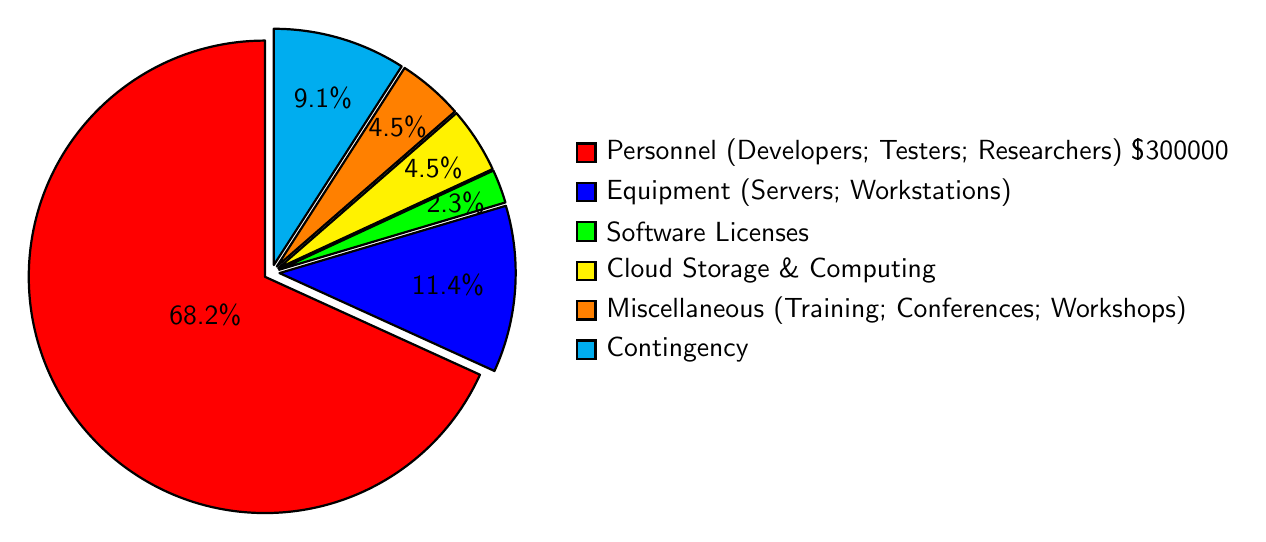
\begin{tikzpicture}
			\pie[rotate=90, explode=0.1, text=legend, 
			radius=3,
			color={red, blue, green, yellow, orange, cyan}]{
				68.2/Personnel (Developers; Testers; Researchers) \$300000,
				11.4/Equipment (Servers; Workstations),
				2.3/Software Licenses,
				4.5/Cloud Storage \& Computing,
				4.5/Miscellaneous (Training; Conferences; Workshops),
				9.1/Contingency
			}
		\end{tikzpicture}
	\end{center}
	
	\newpage
	\section{Conclusion}
	The development of this Large Integer Arithmetic Library, tailored specifically for cryptographic applications, is poised to make a substantial contribution to the field of cryptography. By addressing the inherent limitations of the C language and optimizing for cryptographic needs, this project embodies both innovation and necessity. With a clear timeline, defined milestones, robust data management practices, and a well-structured budget, we are optimistic about the project's success and its subsequent impact on cryptographic research and applications.
	
	1. Final Product or End Goal:
	
	A state-of-the-art Large Integer Arithmetic Library tailored for cryptographic applications, fully integrated with Shanks' Algorithm.
	Comprehensive documentation including user guides, developer notes, and integration guidelines.
	An example application demonstrating the library's capabilities in a real-world cryptographic scenario.
	
	
	SMART Goals:
	
	Specific: Develop a Large Integer Arithmetic Library that can efficiently handle numbers of 256 bits and beyond, specifically optimized for cryptographic tasks, and integrated with Shanks' Algorithm.
	
	Measurable: By the end of Q2 2024, achieve a performance benchmark where the library can perform arithmetic operations on large integers at least 30\% faster than existing generic solutions. Moreover, by the end of the project, gather feedback from at least 50 beta testers, aiming for an approval rating of 85% or higher regarding the library's efficiency and applicability.
	
	Achievable: Assemble a team of experienced developers and cryptography experts, and equip them with the necessary tools and resources, ensuring the project's goals align with their expertise and capabilities.
	
	Relevant: With the growing demand for robust cryptographic solutions in the digital age, developing a specialized library that addresses the inherent limitations of the C language meets a significant market and research need.
	
	Time-bound: Complete the library's development, testing, and documentation within a one-year timeframe, targeting an official launch at the beginning of Q1 2025.
	
	
\end{document}
